\documentclass[preview,border=5pt]{standalone}
\usepackage{teaching}
\begin{document}

\centering
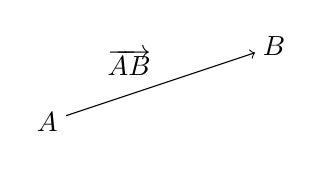
\begin{tikzpicture}[scale=0.8]

\draw [->] (0,0) -- (3,1);
\node at (-0.3,-0.1) {$A$};
\node at (1,0.85) {$\overrightarrow{AB}$};
\node at (3.3,1.1) {$B$};

\end{tikzpicture}

\end{document}